\documentclass[sigplan]{acmart}

\usepackage{booktabs} % For formal tables
\usepackage{graphicx,hyperref}
\usepackage{float}
\usepackage{proof,tikz}
\usepackage{amssymb,amsthm,stmaryrd}


% Copyright
%\setcopyright{none}
%\setcopyright{acmcopyright}
%\setcopyright{acmlicensed}
\setcopyright{rightsretained}
%\setcopyright{usgov}
%\setcopyright{usgovmixed}
%\setcopyright{cagov}
%\setcopyright{cagovmixed}


% DOI
\acmDOI{10.475/123_4}

% ISBN
\acmISBN{123-4567-24-567/08/06}

%Conference
\acmConference[SBLP2018]{XXII BRAZILIAN SYMPOSIUM ON PROGRAMMING LANGUAGES}{September 17--21, 2018}{S\~ao Carlos}
\acmYear{2018}
\copyrightyear{2018}

%\acmPrice{15.00}

%\acmBadgeL[http://ctuning.org/ae/ppopp2016.html]{ae-logo}
%\acmBadgeR[http://ctuning.org/ae/ppopp2016.html]{ae-logo}

%% ODER: format ==         = "\mathrel{==}"
%% ODER: format /=         = "\neq "
%
%
\makeatletter
\@ifundefined{lhs2tex.lhs2tex.sty.read}%
  {\@namedef{lhs2tex.lhs2tex.sty.read}{}%
   \newcommand\SkipToFmtEnd{}%
   \newcommand\EndFmtInput{}%
   \long\def\SkipToFmtEnd#1\EndFmtInput{}%
  }\SkipToFmtEnd

\newcommand\ReadOnlyOnce[1]{\@ifundefined{#1}{\@namedef{#1}{}}\SkipToFmtEnd}
\usepackage{amstext}
\usepackage{amssymb}
\usepackage{stmaryrd}
\DeclareFontFamily{OT1}{cmtex}{}
\DeclareFontShape{OT1}{cmtex}{m}{n}
  {<5><6><7><8>cmtex8
   <9>cmtex9
   <10><10.95><12><14.4><17.28><20.74><24.88>cmtex10}{}
\DeclareFontShape{OT1}{cmtex}{m}{it}
  {<-> ssub * cmtt/m/it}{}
\newcommand{\texfamily}{\fontfamily{cmtex}\selectfont}
\DeclareFontShape{OT1}{cmtt}{bx}{n}
  {<5><6><7><8>cmtt8
   <9>cmbtt9
   <10><10.95><12><14.4><17.28><20.74><24.88>cmbtt10}{}
\DeclareFontShape{OT1}{cmtex}{bx}{n}
  {<-> ssub * cmtt/bx/n}{}
\newcommand{\tex}[1]{\text{\texfamily#1}}	% NEU

\newcommand{\Sp}{\hskip.33334em\relax}


\newcommand{\Conid}[1]{\mathit{#1}}
\newcommand{\Varid}[1]{\mathit{#1}}
\newcommand{\anonymous}{\kern0.06em \vbox{\hrule\@width.5em}}
\newcommand{\plus}{\mathbin{+\!\!\!+}}
\newcommand{\bind}{\mathbin{>\!\!\!>\mkern-6.7mu=}}
\newcommand{\rbind}{\mathbin{=\mkern-6.7mu<\!\!\!<}}% suggested by Neil Mitchell
\newcommand{\sequ}{\mathbin{>\!\!\!>}}
\renewcommand{\leq}{\leqslant}
\renewcommand{\geq}{\geqslant}
\usepackage{polytable}

%mathindent has to be defined
\@ifundefined{mathindent}%
  {\newdimen\mathindent\mathindent\leftmargini}%
  {}%

\def\resethooks{%
  \global\let\SaveRestoreHook\empty
  \global\let\ColumnHook\empty}
\newcommand*{\savecolumns}[1][default]%
  {\g@addto@macro\SaveRestoreHook{\savecolumns[#1]}}
\newcommand*{\restorecolumns}[1][default]%
  {\g@addto@macro\SaveRestoreHook{\restorecolumns[#1]}}
\newcommand*{\aligncolumn}[2]%
  {\g@addto@macro\ColumnHook{\column{#1}{#2}}}

\resethooks

\newcommand{\onelinecommentchars}{\quad-{}- }
\newcommand{\commentbeginchars}{\enskip\{-}
\newcommand{\commentendchars}{-\}\enskip}

\newcommand{\visiblecomments}{%
  \let\onelinecomment=\onelinecommentchars
  \let\commentbegin=\commentbeginchars
  \let\commentend=\commentendchars}

\newcommand{\invisiblecomments}{%
  \let\onelinecomment=\empty
  \let\commentbegin=\empty
  \let\commentend=\empty}

\visiblecomments

\newlength{\blanklineskip}
\setlength{\blanklineskip}{0.66084ex}

\newcommand{\hsindent}[1]{\quad}% default is fixed indentation
\let\hspre\empty
\let\hspost\empty
\newcommand{\NB}{\textbf{NB}}
\newcommand{\Todo}[1]{$\langle$\textbf{To do:}~#1$\rangle$}

\EndFmtInput
\makeatother
%
%
%
%
%
%
% This package provides two environments suitable to take the place
% of hscode, called "plainhscode" and "arrayhscode". 
%
% The plain environment surrounds each code block by vertical space,
% and it uses \abovedisplayskip and \belowdisplayskip to get spacing
% similar to formulas. Note that if these dimensions are changed,
% the spacing around displayed math formulas changes as well.
% All code is indented using \leftskip.
%
% Changed 19.08.2004 to reflect changes in colorcode. Should work with
% CodeGroup.sty.
%
\ReadOnlyOnce{polycode.fmt}%
\makeatletter

\newcommand{\hsnewpar}[1]%
  {{\parskip=0pt\parindent=0pt\par\vskip #1\noindent}}

% can be used, for instance, to redefine the code size, by setting the
% command to \small or something alike
\newcommand{\hscodestyle}{}

% The command \sethscode can be used to switch the code formatting
% behaviour by mapping the hscode environment in the subst directive
% to a new LaTeX environment.

\newcommand{\sethscode}[1]%
  {\expandafter\let\expandafter\hscode\csname #1\endcsname
   \expandafter\let\expandafter\endhscode\csname end#1\endcsname}

% "compatibility" mode restores the non-polycode.fmt layout.

\newenvironment{compathscode}%
  {\par\noindent
   \advance\leftskip\mathindent
   \hscodestyle
   \let\\=\@normalcr
   \let\hspre\(\let\hspost\)%
   \pboxed}%
  {\endpboxed\)%
   \par\noindent
   \ignorespacesafterend}

\newcommand{\compaths}{\sethscode{compathscode}}

% "plain" mode is the proposed default.
% It should now work with \centering.
% This required some changes. The old version
% is still available for reference as oldplainhscode.

\newenvironment{plainhscode}%
  {\hsnewpar\abovedisplayskip
   \advance\leftskip\mathindent
   \hscodestyle
   \let\hspre\(\let\hspost\)%
   \pboxed}%
  {\endpboxed%
   \hsnewpar\belowdisplayskip
   \ignorespacesafterend}

\newenvironment{oldplainhscode}%
  {\hsnewpar\abovedisplayskip
   \advance\leftskip\mathindent
   \hscodestyle
   \let\\=\@normalcr
   \(\pboxed}%
  {\endpboxed\)%
   \hsnewpar\belowdisplayskip
   \ignorespacesafterend}

% Here, we make plainhscode the default environment.

\newcommand{\plainhs}{\sethscode{plainhscode}}
\newcommand{\oldplainhs}{\sethscode{oldplainhscode}}
\plainhs

% The arrayhscode is like plain, but makes use of polytable's
% parray environment which disallows page breaks in code blocks.

\newenvironment{arrayhscode}%
  {\hsnewpar\abovedisplayskip
   \advance\leftskip\mathindent
   \hscodestyle
   \let\\=\@normalcr
   \(\parray}%
  {\endparray\)%
   \hsnewpar\belowdisplayskip
   \ignorespacesafterend}

\newcommand{\arrayhs}{\sethscode{arrayhscode}}

% The mathhscode environment also makes use of polytable's parray 
% environment. It is supposed to be used only inside math mode 
% (I used it to typeset the type rules in my thesis).

\newenvironment{mathhscode}%
  {\parray}{\endparray}

\newcommand{\mathhs}{\sethscode{mathhscode}}

% texths is similar to mathhs, but works in text mode.

\newenvironment{texthscode}%
  {\(\parray}{\endparray\)}

\newcommand{\texths}{\sethscode{texthscode}}

% The framed environment places code in a framed box.

\def\codeframewidth{\arrayrulewidth}
\RequirePackage{calc}

\newenvironment{framedhscode}%
  {\parskip=\abovedisplayskip\par\noindent
   \hscodestyle
   \arrayrulewidth=\codeframewidth
   \tabular{@{}|p{\linewidth-2\arraycolsep-2\arrayrulewidth-2pt}|@{}}%
   \hline\framedhslinecorrect\\{-1.5ex}%
   \let\endoflinesave=\\
   \let\\=\@normalcr
   \(\pboxed}%
  {\endpboxed\)%
   \framedhslinecorrect\endoflinesave{.5ex}\hline
   \endtabular
   \parskip=\belowdisplayskip\par\noindent
   \ignorespacesafterend}

\newcommand{\framedhslinecorrect}[2]%
  {#1[#2]}

\newcommand{\framedhs}{\sethscode{framedhscode}}

% The inlinehscode environment is an experimental environment
% that can be used to typeset displayed code inline.

\newenvironment{inlinehscode}%
  {\(\def\column##1##2{}%
   \let\>\undefined\let\<\undefined\let\\\undefined
   \newcommand\>[1][]{}\newcommand\<[1][]{}\newcommand\\[1][]{}%
   \def\fromto##1##2##3{##3}%
   \def\nextline{}}{\) }%

\newcommand{\inlinehs}{\sethscode{inlinehscode}}

% The joincode environment is a separate environment that
% can be used to surround and thereby connect multiple code
% blocks.

\newenvironment{joincode}%
  {\let\orighscode=\hscode
   \let\origendhscode=\endhscode
   \def\endhscode{\def\hscode{\endgroup\def\@currenvir{hscode}\\}\begingroup}
   %\let\SaveRestoreHook=\empty
   %\let\ColumnHook=\empty
   %\let\resethooks=\empty
   \orighscode\def\hscode{\endgroup\def\@currenvir{hscode}}}%
  {\origendhscode
   \global\let\hscode=\orighscode
   \global\let\endhscode=\origendhscode}%

\makeatother
\EndFmtInput
%

\DeclareMathAlphabet{\mathkw}{OT1}{cmss}{bx}{n}


\newcommand{\EvalCtxTran}[1]{\ensuremath{\mathbb{T}[#1]}}
\newcommand{\EvalCtxProc}[1]{\ensuremath{\mathbb{P}[#1]}}

\newtheorem{Lemma}{Lemma}
\newtheorem{Theorem}{Theorem}
\theoremstyle{definition}
\newtheorem{Example}{Example}


\usepackage{color}
\newcommand{\redFG}[1]{\textcolor[rgb]{0.6,0,0}{#1}}
\newcommand{\greenFG}[1]{\textcolor[rgb]{0,0.4,0}{#1}}
\newcommand{\blueFG}[1]{\textcolor[rgb]{0,0,0.8}{#1}}
\newcommand{\orangeFG}[1]{\textcolor[rgb]{0.8,0.4,0}{#1}}
\newcommand{\purpleFG}[1]{\textcolor[rgb]{0.4,0,0.4}{#1}}
\newcommand{\yellowFG}[1]{\textcolor{yellow}{#1}}
\newcommand{\brownFG}[1]{\textcolor[rgb]{0.5,0.2,0.2}{#1}}
\newcommand{\blackFG}[1]{\textcolor[rgb]{0,0,0}{#1}}
\newcommand{\whiteFG}[1]{\textcolor[rgb]{1,1,1}{#1}}
\newcommand{\yellowBG}[1]{\colorbox[rgb]{1,1,0.2}{#1}}
\newcommand{\brownBG}[1]{\colorbox[rgb]{1.0,0.7,0.4}{#1}}

\newcommand{\ColourStuff}{
  \newcommand{\red}{\redFG}
  \newcommand{\green}{\greenFG}
  \newcommand{\blue}{\blueFG}
  \newcommand{\orange}{\orangeFG}
  \newcommand{\purple}{\purpleFG}
  \newcommand{\yellow}{\yellowFG}
  \newcommand{\brown}{\brownFG}
  \newcommand{\black}{\blackFG}
  \newcommand{\white}{\whiteFG}
}

\newcommand{\MonochromeStuff}{
  \newcommand{\red}{\blackFG}
  \newcommand{\green}{\blackFG}
  \newcommand{\blue}{\blackFG}
  \newcommand{\orange}{\blackFG}
  \newcommand{\purple}{\blackFG}
  \newcommand{\yellow}{\blackFG}
  \newcommand{\brown}{\blackFG}
  \newcommand{\black}{\blackFG}
  \newcommand{\white}{\blackFG}
}

\ColourStuff

\newcommand{\D}[1]{\blue{\mathsf{#1}}}
\newcommand{\C}[1]{\red{\mathsf{#1}}}
\newcommand{\F}[1]{\green{\mathsf{#1}}}
\newcommand{\V}[1]{\black{\mathsf{#1}}}
\newcommand{\TC}[1]{\purple{\mathsf{#1}}}


\newcommand{\TStep}[9]{\ensuremath{\langle  #2, #3, #4 \rangle
    \mapsto_{T_{#5}} \langle  #7, #8, #9 \rangle}}


\begin{document}

\title{A Property Based Testing Approach for Software Transactional Memory Safety}

\author{Rodrigo Ribeiro}
\affiliation{
  \institution{Universidade Federal de Ouro Preto}
  \city{Ouro Preto} 
  \state{Minas Gerais}
  \country{Brazil}
}

\author{Andr\'e Du Bois}
\affiliation{
  \institution{Universidade Federal de Pelotas}
  \city{Pelotas}
  \state{Rio Grande do Sul}
  \country{Brazil}
} 

\begin{abstract}
Software Transactional Memory (STM) provides programmers with a simple high-level model of transactions that allows the
writing of concurrent programs without worrying with locks, since all transaction concurrency management is done by
the STM runtime. Such programming model greatly simplifies development of concurrent applications, but it has a cost:
implementing an efficient and correct STM algorithm is an art. Several criteria have been proposed to certify
STM algorithms, some based on model checkers and proof assistants. Such approaches are heavyweight and
do not allow quick experimentation with different TM algorithm designs. In this work, we propose a more
lightweight approach: specify STM algorithm as small-step operational semantics of a idealized language with
STM support and check for safety properties using QuickCheck, a property-based testing library for Haskell.
\end{abstract}

\begin{CCSXML}\begin{hscode}\SaveRestoreHook
\column{B}{@{}>{\hspre}l<{\hspost}@{}}%
\column{E}{@{}>{\hspre}l<{\hspost}@{}}%
\>[B]{}\V{ccs2012}\mathbin{>}{}\<[E]%
\\
\>[B]{}\V{concept}\mathbin{>}{}\<[E]%
\\
\>[B]{}\V{concept\char95 id}\mathbin{>}\C{10003752.10010124}\mathbin{\circ}\C{10010131.10010134}\mathbin{</}\V{concept\char95 id}\mathbin{>}{}\<[E]%
\\
\>[B]{}\V{concept\char95 desc}\mathbin{>}\V{Theory}\;\mathkw{of}\;\V{computation}\mathord{\sim}\V{Operational}\;\V{semantics}\mathbin{</}\V{concept\char95 desc}\mathbin{>}{}\<[E]%
\\
\>[B]{}\V{concept\char95 significance}\mathbin{>}\C{500}\mathbin{</}\V{concept\char95 significance}\mathbin{>}{}\<[E]%
\\
\>[B]{}\mathbin{/}\V{concept}\mathbin{>}{}\<[E]%
\\
\>[B]{}\V{concept}\mathbin{>}{}\<[E]%
\\
\>[B]{}\V{concept\char95 id}\mathbin{>}\C{10011007.10011006}\mathbin{\circ}\C{10011008.10011009}\mathbin{\circ}\C{10011014}\mathbin{</}\V{concept\char95 id}\mathbin{>}{}\<[E]%
\\
\>[B]{}\V{concept\char95 desc}\mathbin{>}\V{Software}\;\V{and}\;\V{its}\;\V{engineering}\mathord{\sim}\V{Concurrent}\;\V{programming}\;\V{languages}\mathbin{</}\V{concept\char95 desc}\mathbin{>}{}\<[E]%
\\
\>[B]{}\V{concept\char95 significance}\mathbin{>}\C{500}\mathbin{</}\V{concept\char95 significance}\mathbin{>}{}\<[E]%
\\
\>[B]{}\mathbin{/}\V{concept}\mathbin{>}{}\<[E]%
\\
\>[B]{}\mathbin{/}\V{ccs2012}\mathbin{>}{}\<[E]%
\ColumnHook
\end{hscode}\resethooks
\end{CCSXML}

\ccsdesc[500]{Theory of computation~Operational semantics}
\ccsdesc[500]{Software and its engineering~Concurrent programming languages}


\maketitle

\section{Introduction}

Transactional Memory (TM)~\cite{Herlihy1993,Shavit1995} provides programmers a high level concurrency
control abstraction. Programmers can simply declare certain code pieces as
transactions and the TM runtime guarantees that transactions execute in isolation.
The use of TM provides atomicity, deadlock freedom, composability~\cite{Harris05} and
increases productivity when compared to using locks~\cite{Pankratius2011}. Several works developed
software~\cite{Herlihy2003,Herlihy2006,Dice06}, hardware~\cite{Hammond2004} and software / hardware hybrids~\cite{Baugh2008,Dalessandro2011}
implementations. Gradually, industry is adopting TM: IBM Blue Gene/Q processor supports TM and Intel Haswell microarchitecture
supports transaction synchronization primitives~\cite{TSX,Haring2012}.

The TM runtime is responsible to ensure correct management of shared state. Therefore,
correctness of TM clients depend on a correct implementation of TM algorithms. However,
this simple programming model has a price: designing a correct TM algorithm is an art.
Researchers use different techniques to implement the TM interface efficiently. Algorithms
try to interleave transactions as much as possible, while guaranteeing a non-interleaving
semantics. Thus, subtle but fast algorithms are favored over simpler ones and such subtlety
makes them prone to intricate bugs.


A first step towards correct implementation of TM algorithms is a specification of what
is correctness for TM. Intuitively, a correct TM algorithm should guarantee that every
execution of an arbitrary set of transactions is indistinguishable from a sequential
running of them. Several correctness criteria where proposed in the
literature~\cite{Guerraoui2008,Doherty2009,Imbs2009,LesaniP14} and
they rely on the concept of transactional histories. Intuitively,
a history consists of a sequence of operations executed on shared objects
during a TM execution. Analysing TM history structure generated by algorithms,
we can ensure that its TM interface provides atomicity and deadlock freedom to client
applications. However, certify that a TM algorithm is safe according to some criteria
is a non-trivial task. Different works use I/O automata~\cite{Lesani2012}, model
checking~\cite{CohenPZ08,cohen2007,Guerraoui2008a} or define a specification language that
reduces the problem of proving non-opacity of a TM algorithm to SMT solving~\cite{Lesani2013,DeMoura2008}.

Such correctness concerns are not just formalization curiosity, they can influence directly on implementation efficiency.
Le et.al.~\cite{Le2016} mention that current STM-Haskell implementation does not enjoy opacity and that it
can cause threads to loop, due to accessing an inconsistent memory view. To avoid such problems STM-Haskell
implementation validates the read set each time a thread is scheduled and such checking overhead can cause
a waste of execution time. This is one of the motivation for Le et. al.~\cite{Le2016} proposing a new
implementation of STM-Haskell using the Transaction Locking II (TL2) algorithm~\cite{Dice06}. 

Defining formal semantics and correctness criteria are fundamental steps to ensure safety of TM algorithms.
To the best of our knowledge, there is no truly small-step semantics for TM such that: 1) consider high-level constructs like \ensuremath{\F{orElse}}
and \ensuremath{\F{retry}} while allowing the interleaving of executing transactions and 2) produces a history of TM execution that can be used to verify
safety of TM semantics. This work aims to fill this gap. Our approach is to specify STM algorithms
using a standard small-step operational semantics
for a simple transactional language and use property based testing to check if safety properties are satisified by histories generated.
We are aware that using automated testing isn't sufficient to ensure correctness of an algorithm, but
it can expose bugs before using more formal approaches, like formalizing the algorithm in a proof assistant.

Specifically, we made the following contributions:

\begin{itemize}
   \item We define a simplified model language that supports high-level TM constructs 
         \ensuremath{\F{orElse}} and \ensuremath{\F{retry}} present in STM-Haskell.
   \item We define two trace based small-step operational semantics for a high-level 
         language with STM support. One semantics closely follows the well-known TL2
         algorithm~\cite{Dice06} and the other is based on the semantics adopted by STM Haskell~\cite{Harris05}.
         These semantics are implemented in the Haskell programming language.
   \item We define TM safety condition, namely opacity~\cite{Guerraoui2008},
         in Haskell and check them using QuickCheck~\cite{Claessen00} against
         the implemented semantics. Defining safety properties is just a matter to define functions
         that verify them on histories produced by interpreters implementing TM algorithm
         semantics.
\end{itemize}

The rest of this paper is organized as follows.  Section \ref{sec:stm-model}
defines the syntax (Section \ref{sec:stm-syntax}) and operational semantics
based on TL2 and on STM-Haskell (Section \ref{sec:stm-semantics}) for a small STM-Haskell like language.
In Section \ref{sec:stm-safety}
we present Haskell implementation of opacity safety property and describe how to check it using
QuickCheck, giving some details on how random test cases are generated and presenting test coverage results.
Section \ref{sec:related} discuss related work and Section \ref{sec:conclusion} concludes and
presents future work.

We assume that the reader knows the Haskell programming language~\cite{Lipovaca2011}.
All source code produced, including the literate Haskell source of this article
(which can be preprocessed using lhs2\TeX~\cite{Loh2005}), instructions on how to
build it and reproduce the developed test suit are avaliable on-line~\cite{stm-rep}.



% All code described in this paper was developed using GHC-8.0.1 and it is available on-line~\cite{}.

\section{A Model for Software Transactional Memory}\label{sec:stm-model}

Our objective is to formalize semantic that ensure, by construction, that an
implementation for transactional memory enjoy opacity. 

\subsection{Language Syntax}\label{sec:stm-syntax}

Our minimalistic language is defined by data types \ensuremath{\D{Tran}}, which
represents computations in the \ensuremath{\D{STM}} monad, and \ensuremath{\D{Proc}} that denotes
actions in the Haskell \ensuremath{\D{IO}} monad. This language is, in essence,
the same as the one proposed by~\cite{Hu08}. We extend it with
\ensuremath{\F{orElse}}, \ensuremath{\F{retry}}, conditional constructs and a special value to
denote a aborted transaction, \ensuremath{\C{TAbort}}. Such constructs aren't
an essential part of a model for TM, but they interesting
on their own when we consider safety properties of TM.

\begin{hscode}\SaveRestoreHook
\column{B}{@{}>{\hspre}l<{\hspost}@{}}%
\column{E}{@{}>{\hspre}l<{\hspost}@{}}%
\>[B]{}\mathkw{newtype}\;\D{Val}\mathrel{=}\D{Val}\;\{\mskip1.5mu \C{ unVal }\mathbin{::}\D{Int}\mskip1.5mu\}{}\<[E]%
\\[\blanklineskip]%
\>[B]{}\mathkw{newtype}\;\D{Var}\mathrel{=}\D{Var}\;\{\mskip1.5mu \C{ unVar }\mathbin{::}\D{Int}\mskip1.5mu\}{}\<[E]%
\\[\blanklineskip]%
\>[B]{}\mathkw{newtype}\;\D{Id}\mathrel{=}\D{Id}\;\{\mskip1.5mu \C{unId}\mathbin{::}\D{Int}\mskip1.5mu\}{}\<[E]%
\\[\blanklineskip]%
\>[B]{}\mathkw{data}\;\D{Tran}\mathrel{=}\C{TVal}\;\D{Val}\mid \C{TRead}\;\D{Var}\mid \C{TWrite}\;\D{Var}\;\D{Tran}{}\<[E]%
\\
\>[B]{}\mid \D{Tran}\C{\,\oplus_T\,}\D{Tran}\mid \C{TIf}\;\D{Tran}\;\D{Tran}\;\D{Tran}{}\<[E]%
\\
\>[B]{}\mid \C{TOrElse}\;\D{Tran}\;\D{Tran}\mid \C{TRetry}\mid \C{TAbort}{}\<[E]%
\\[\blanklineskip]%
\>[B]{}\mathkw{data}\;\D{Proc}\mathrel{=}\C{PVal}\;\D{Val}\mid \C{PFork}\;\D{Proc}{}\<[E]%
\\
\>[B]{}\mid \C{PAt}\;(\D{Maybe}\;(\D{Id},\D{Stamp}))\;\D{Tran}{}\<[E]%
\\
\>[B]{}\mid \D{Proc}\C{\,\oplus_P\,}\D{Proc}{}\<[E]%
\ColumnHook
\end{hscode}\resethooks

In order to avoid dealing with name binding, we do
not provide a language construct for creating new
variables and also use addition operation for
composing transactions and processes. This is valid simplification,
since addition forms a monoid on integer values, while still retaining
the sequencing computations and combining their results\footnote{This is valid since a monoid can be seen as a degenerate case of a monad.}.
We represent variables and values by integers (properly
wrapped using a \ensuremath{\mathkw{newtype}}). Each syntax construct meaning
is immediate with the exception of how we represent atomic blocks. A value built with constructor
\ensuremath{\C{PAt}} carries information about its transaction id and current
transaction read stamp. Initially, all \ensuremath{\C{PAt}} values are built using
\ensuremath{\C{Nothing}} to denote that such block did not started its execution.
To avoid clutter in the presentation of \ensuremath{\C{PAt}} semantics, we represent
information about transaction id and read stamp as $(i,j)$ whenever it
has the form \ensuremath{\C{Just}} $(i,j)$ and as $()$ if it is equal to \ensuremath{\C{Nothing}}. Also,
we allow ourselves a bit of informality and write \ensuremath{\D{Id}}s, \ensuremath{\D{Stamp}}s, \ensuremath{\D{Val}}
and \ensuremath{\D{Var}} values as if they were simple integers.

Construction \ensuremath{\C{TAbort}} is used to represent a transaction
that is aborted by accessing an inconsistent view of memory,
in our TL2-based semantics, and by trying to commit an transaction that
which has accessed and invalid memory configuration, in STM-Haskell based semantics.
Term \ensuremath{\C{TAbort}} does not appear on randomly
generated source programs.
It is used in our semantics to properly
differ between different types of transaction aborting and how
they should be treated by semantics of \ensuremath{\F{orElse}} construct, since
transactions aborted by inconsistent views should not be captured
by an \ensuremath{\F{orElse}}.


\subsection{Language Semantics}\label{sec:stm-semantics}

In this section, we define two operational semantics for our STM language. First, we
present a semantics inspired by the TL2 algorithm which unlike previous works~\cite{Harris05,Hu08}
uses heaps, transaction logs (read and write sets) and also records the event history of current
TM execution. The use of transaction logs on a high-level semantics is a bit unusual, but necessary
to proper modeling of commit and abort operations of different TM algorithms. Next, we propose a
semantics inspired by STM Haskell in which no global clock is used for \ensuremath{\D{TVar}} version control.

%Following common practice, notation $h\,[x\mapsto v]$ denotes
%finite mapping update, i.e. finite mapping $h'$ such that:
%1) $h'(x) = v$ and 2) $h'(y) = h(y)$, for $x \neq y$.
%To avoid notation clutter, w

Before presenting the semantics, we need to define some notation.
We use finite maps to  represent heaps and logs used by transactions (i.e. read and write
sets). Notation $\bullet$ denotes an empty finite mapping and
$\Theta$ represents a 4-uple formed by a heap and mappings between transaction id's and their
read / write sets and transactions. We let $\Theta_h$, $\Theta_r$, $\Theta_w$, and $\Theta_T$ represent the heap and finite
functions between transaction ids and their logs and transactions,
respectively. Let $h(x)$ denote the operation
of retrieving the value associated with key $x$ in finite mapping 
$h$ and $h(x)=\bot$ denotes that no value is associated
with $x$. Notation $h \uplus h'$ denotes the right-biased union of 
two finite mappings, i.e. when both maps have the same key $x$, we keep
the value $h'(x)$. We let $\Theta_r(x,j)$ denote the operation of
retrieving the value associated with key $x$ in the read set of transaction
with id $j$. Notation $\Theta_w(x,j)$ is defined similarly for write sets. Updating
a variable $x$ with value $v$ in the read set of transaction $j$ is denoted as
$\Theta_r\,[j,x\mapsto v]$. Same holds for write set $\Theta_w$.
Finally, notation $h\mid_{x}$ denotes the finite mapping $h'$ with entries for the key $x$
removed, i.e. $h' = h - [ x \mapsto v]$, for some value $v$.


Operations executed on transactional variables during a TM
execution are represented by data type \ensuremath{\D{Event}}. Essentially,
\ensuremath{\D{Event}} records operations on variables and on transactions.
A history of a TM execution is formed by a list of \ensuremath{\D{Event}}s.
\begin{hscode}\SaveRestoreHook
\column{B}{@{}>{\hspre}l<{\hspost}@{}}%
\column{11}{@{}>{\hspre}l<{\hspost}@{}}%
\column{E}{@{}>{\hspre}l<{\hspost}@{}}%
\>[B]{}\mathkw{newtype}\;\D{Stamp}\mathrel{=}\D{Stamp}\;\{\mskip1.5mu \C{ unStamp }\mathbin{::}\D{Int}\mskip1.5mu\}{}\<[E]%
\\[\blanklineskip]%
\>[B]{}\mathkw{data}\;\D{Event}\mathrel{=}\C{IRead}\;\D{Id}\;\D{Var}\;\D{Val}\mid \C{IWrite}\;\D{Id}\;\D{Var}\;\D{Val}{}\<[E]%
\\
\>[B]{}\hsindent{11}{}\<[11]%
\>[11]{}\mid \C{IBegin}\;\D{Id}\mid \C{ICommit}\;\D{Id}\mid \C{IAbort}\;\D{Id}\mid \C{IRetry}\;\D{Id}{}\<[E]%
\\[\blanklineskip]%
\>[B]{}\mathkw{type}\;\D{History}\mathrel{=}[\mskip1.5mu \D{Event}\mskip1.5mu]{}\<[E]%
\ColumnHook
\end{hscode}\resethooks
Data type \ensuremath{\D{Stamp}} denotes the global clock used by the TL2 algorithm to ensure correct variable versions.
Constructors \ensuremath{\C{IBegin}}, \ensuremath{\C{ICommit}} and \ensuremath{\C{IAbort}} denote the beginning, commit and failure of
a transaction with a given \ensuremath{\D{Id}}. We consider that a transaction fails
when it tries to read from an inconsistent view of memory. \ensuremath{\C{IRead}\;\V{id}\;\V{v}\;\V{val}} records that
value \ensuremath{\V{val}} was read by transaction \ensuremath{\V{id}} for variable \ensuremath{\V{v}} and \ensuremath{\C{IWrite}\;\V{id}\;\V{v}\;\V{val}}
denotes that value \ensuremath{\V{val}} was written in variable \ensuremath{\V{v}} by transaction \ensuremath{\V{id}}.
An event \ensuremath{\C{IRetry}} denotes the user called \ensuremath{\F{retry}} on current transaction and such
transaction should be restarted. In our semantics, the computation of histories is represented
as a Writer monad, which adds a new element by appending at history end. But, for presentation
purpouses, we simply add a new event at head of a given history.

\subsubsection{TL2 Based Semantics}

Now, we present our semantics based on Transactional Locking 2 
algorithm~\cite{Dice06}. Informally, TL2 algorithm works as follows:
threads execute reads and writes to objects, but no memory locations are actually modified. All 
writes and reads are recorded in write and read logs. When a
transaction finishes, it validates its log to check if it has seen a 
consistent view of memory, and its changes are committed to memory.

Function $\Theta(x,i,j)$ denotes that transaction $j$ with read-stamp $i$ tries to
to read the content of variable $x$ and it works as follows:
First it checks the write set. If the variable has not been written to, the read set is consulted.
Otherwise, if the variable has also not been read, its value is looked up from the heap and the read log updated accordingly, if
variable's write stamp is not greater than current transaction read-stamp $i$. Otherwise, we have an conflict and the current
transaction is aborted by returning \ensuremath{\C{TAbort}}.

\begin{figure}[h]
  \[
  \Theta(x,i,j) = \left\{
  \begin{array}{ll}
     (v,\Theta) & \textit{if }\:\Theta_w(x,j) = (i',v)\\
     (v,\Theta) & \textit{if }\:\Theta_w(x,j) = \bot,\Theta_r(x,j) \neq \bot, \\
                & \:\:\:\:\: \Theta_h(x) = (i',v) \textit{ and } i \geq i'\\
     (v, \Theta_r\,[j,x \mapsto v]) & 
        \textit{if }\:\Theta_w(x) = \Theta_r(x) = \bot,\\
                                       & \:\:\:\:\:  \Theta_h(x) = (i',v),
                                     \textit{ and } i \geq i' \\
                           \ensuremath{\C{TAbort}} & \textit{if }\: \Theta_h(x) = (i',v)
                                    \textit{ and } i < i'
  \end{array}
                                  \right.
  \]
  \centering
  \caption{Reading a variable}
  \label{fig:readvar}
\end{figure}

Predicate $consistent(\Theta,i,j)$ holds if transaction $j$ has finished its execution
on a valid view of memory. We say that a TM state $\Theta$ is consistent if all variables read
have stamps less than or equal to $i$, the global clock value in which transaction $j$ have started.

\begin{figure}[h]
  \[
     consistent(\Theta,i,j) = \forall x. \Theta_r(x,j) = (i,v) \to
     \Theta_h(x) = (i',v) \land i \geq i'
  \]
  \centering
  \caption{Predicate for consistency of transaction logs}
  \label{fig:consistency}
\end{figure}


In order to provide a concise semantics definition, in Figure~\ref{fig:hole-syntax},
we define evaluation contexts to avoid the need of ``congruence rules''. In our
semantics definition we use the following meta-variable convention: we let $t$
denote arbitrary transactions and $p$ processes. Values are represented by $v$,
stamps by $i$ and transaction ids by $j$. All meta-variables can appear primed or subscripted, as
usual. Finally, in order to avoid several rules to propagating different types of
transaction failure, we use \ensuremath{\C{TFail}} whenever any of \ensuremath{\C{TAbort}} or \ensuremath{\C{TRetry}} applies.
Same holds for events: \ensuremath{\C{IFail}} will represent any of \ensuremath{\C{IAbort}} or \ensuremath{\C{IRetry}}.  

\begin{figure}[h]
        \[
            \begin{array}{cc}
               \begin{array}{c}
                   \textit{Contexts for transactions} \\
                   \\
                   \begin{array}{rcl}
                      \EvalCtxTran{\cdot} & ::=    & \ensuremath{\C{TWrite}}\, v\:\EvalCtxTran{\cdot}\\
                                                   & \mid &\EvalCtxTran{\cdot}\: \ensuremath{\C{\,\oplus_T\,}} t\\
                                                   & \mid & \ensuremath{\C{TVal}}\,v \ensuremath{\C{\,\oplus_T\,}} \EvalCtxTran{\cdot}\\
                                                   & \mid & \ensuremath{\C{TIf}}\:\EvalCtxTran{\cdot}\:t\:t' \\
                                                   & \mid & \ensuremath{\C{TOrElse}}\:\EvalCtxTran{\cdot}\:t\\
                   \end{array}
               \end{array}
               &
               \begin{array}{c}
                    \textit{Contexts for processes}\\
                    \\
                    \begin{array}{rcl}
                      \EvalCtxProc{\cdot} & ::=    & \ensuremath{\C{PFork}}\:\EvalCtxProc{\cdot}\\
                                                   & \mid &\EvalCtxProc{\cdot}\:\ensuremath{\C{\,\oplus_P\,}} t\\
                                                   & \mid & \ensuremath{\C{PVal}}\,v\,\ensuremath{\C{\,\oplus_P\,}}\EvalCtxProc{\cdot}\\
                                                   & \mid & \ensuremath{\C{PAt}}\,(\ensuremath{\C{Just}}\, (i,j))\:\EvalCtxProc{\cdot}
                    \end{array}
               \end{array}
            \end{array}
        \]
        \centering
        \caption{Evaluation contexts for high-level language.}
        \label{fig:hole-syntax}
\end{figure}

\paragraph{Transaction Semantics:}

We define transaction semantics by a reduction relation $\mapsto_{T_{i\,j}}$ on triples
$\langle \Theta, \sigma, t \rangle$, where $\Theta$ is the current state of TM,
$\sigma$ is the history of TM execution and $t$ is a transaction. Variables $i$ and $j$
denote the current transaction read stamp and id, respectively. First, we present
the rule used to evaluate transaction contexts.

\[
  \infer[_{(TContext)}]
        { \langle \Theta,\,\sigma,\,\EvalCtxTran{t}\rangle \mapsto_{T_{i\,j}}
          \langle \Theta',\,\sigma',\,\EvalCtxTran{t'}\rangle }
        { \langle \Theta,\,\sigma,\,t \rangle \mapsto_{T_{i\,j}}
          \langle \Theta',\,\sigma',\, t'\rangle }
\]

This rule simply allows stepping some subterm of current transaction expression $\EvalCtxTran{t}$.

Next, we will consider how to evaluate a \ensuremath{\C{TRead}} construct. Notice that, 
we need two different rules for reading variables. This happens because, in our semantics, the
function that reads a value from a variable can abort the current transaction, as it happens in TL2,
if its write stamp is less than current transactions read stamp.

\[
\begin{array}{c}
  \infer[_{(TReadOk)}]
        { \langle \Theta,\, \sigma, \ensuremath{\C{TRead}}\,v \rangle \mapsto_{T_{i\,j}}
          \langle \Theta',\, \sigma',\,\ensuremath{\C{TVal}}\,val\rangle }
        {\Theta(v,i,j) = (val,\Theta') & \sigma' = \ensuremath{\C{IRead}}\,j\,v\,val\,:\sigma}
  \\
  \\
  \infer[_{(TReadFail)}]
        { \langle \Theta,\, \sigma, \ensuremath{\C{TRead}}\,v \rangle \mapsto_{T_{i\,j}}
          \langle \Theta, \, \sigma',\, \ensuremath{\C{TAbort}} \rangle}
        {\Theta(v,i,j) = (\ensuremath{\C{TAbort}},\Theta') & \sigma' = \ensuremath{\C{IAbort}}\,j\,:\sigma} 
\end{array}
\]

Writing a value is done by next rules: rule $(TWriteVal)$ writes a completely
reduced value and rule $(TWriteFail)$ just does propagate failure for
signaling that current transaction has failed or aborted throught an explicit
\ensuremath{\C{TRetry}}.

\[
\begin{array}{c}
  \infer[_{(TWriteVal)}]
        { \langle \Theta, \, \sigma, \ensuremath{\C{TWrite}}\,v\,(\ensuremath{\C{TVal}}\,val)\rangle \mapsto_{T_{i\,j}}
          \langle \Theta', \, \sigma',\,\ensuremath{\C{TVal}}\,val\rangle}
        {\begin{array}{c}
            \Theta' = \langle \Theta_h, \Theta_r, \Theta_w[j,x \mapsto val], \Theta_T\rangle \\
            \sigma' = \ensuremath{\C{IWrite}}\,j\,v\,val\, : \sigma \\
         \end{array}}
  \\ \\
  \infer[_{(TWriteFail)}]
        { \langle \Theta, \,\sigma, \ensuremath{\C{TWrite}}\,v\,\ensuremath{\C{TFail}}\rangle \mapsto_{T_{i\,j}}
          \langle \Theta, \, \sigma,\, \ensuremath{\C{TFail}} \rangle }
        { }
\end{array}
\]

Since we replace monadic bind by addition, we need to
force a sequential order of evaluation and some additional
rules to ensure the correct propagation of
failure.

\[
\begin{array}{c}
  \infer[_{(TAddVal)}]
        { \langle \Theta, \, \sigma,\, (\ensuremath{\C{TVal}}\,val_1) \ensuremath{\C{\,\oplus_T\,}} (\ensuremath{\C{TVal}}\,val_2) \rangle \mapsto_{T_{i\,j}}
          \langle \Theta, \, \sigma,\, \ensuremath{\C{TVal}}\,val \rangle}
        {val = val_1 + val_2}
  \\ \\
  \infer[_{(TAddL)}]
        { \langle \Theta,\,\sigma,\,\ensuremath{\C{TFail}}\,\ensuremath{\C{\,\oplus_T\,}} t\rangle \mapsto_{T_{i\,j}}
          \langle \Theta',\,\sigma', \ensuremath{\C{TFail}}\rangle}
        { }

%\langle \Theta,\,\sigma,\,t\rangle \mapsto_{T_{i\,j}}
%         \langle \Theta',\,\sigma',\,|TFail|\rangle 

  \\ \\
  \infer[_{(TAddR)}]
        { \langle \Theta,\,\sigma,\, (\ensuremath{\C{TVal}}\, val) \ensuremath{\C{\,\oplus_T\,}} \ensuremath{\C{TFail}} \rangle \mapsto_{T_{i\,j}}
          \langle \Theta',\,\sigma',\,\ensuremath{\C{TFail}} \rangle }
        { }
\end{array}
\]

We can evaluate a \ensuremath{\C{TIf}} to its first branch if its condition is equal to zero or to its
second otherwise. 

\[
  \begin{array}{c}
     \infer[_{(TIfZero)}]
           {\langle \Theta,\sigma,\ensuremath{\C{TIf}}\,(\ensuremath{\C{TVal}\;\C{0}})\,t\,t'\rangle \mapsto_{T_{i\,j}}
            \langle \Theta,\sigma,\,t\rangle}
           {}
     \\ \\
     \infer[_{(TIfNonZero)}]
           {\langle \Theta,\sigma,\ensuremath{\C{TIf}}\,(\ensuremath{\C{TVal}\;\V{v}})\,t\,t'\rangle \mapsto_{T_{i\,j}}
            \langle \Theta,\sigma,\,t'\rangle}
           {v \neq 0}          
  \end{array}
\]

We also propagate failures produced on \ensuremath{\C{TIf}} condition evaluation.

\[
  \begin{array}{c}
     \infer[_{(TIfFail)}]
           { \langle \Theta,\,\sigma,\,\ensuremath{\C{TIf}}\,\ensuremath{\C{TFail}}\,t\,t'\rangle\mapsto_{T_{i\,j}}
             \langle \Theta,\,\sigma,\,\ensuremath{\C{TFail}}\rangle }
           {}
  \end{array}
\]

Evaluating a \ensuremath{\C{TOrElse}} construct returns a value, if whenever its left transaction
reduces to \ensuremath{\C{TVal}\;\V{v}}. Right transaction is executed only when the left one reduces to
\ensuremath{\C{TRetry}}. Finally, if a transaction aborts such aborting signal is propagated.

\[
  \begin{array}{c}
     \infer[_{(TOrElseVal)}]
           { \langle \Theta,\,\sigma,\,\ensuremath{\C{TOrElse}}\,(\ensuremath{\C{TVal}}\:v)\,t'\rangle \mapsto_{T_{i\,j}}
             \langle \Theta',\,\sigma',\,\ensuremath{\C{TVal}}\,v \rangle }
           {  }
     \\ \\
     \infer[_{(TOrElseR)}]
           { \langle \Theta,\,\sigma,\,\ensuremath{\C{TOrElse}}\,\ensuremath{\C{TRetry}}\,t'\rangle \mapsto_{T_{i\,j}}
             \langle \Theta,\,\sigma,\,t' \rangle }
           { }
      \\ \\
     \infer[_{(TOrElseA)}]
           { \langle \Theta,\,\sigma,\,\ensuremath{\C{TOrElse}}\,\ensuremath{\C{TAbort}}\,t'\rangle \mapsto_{T_{i\,j}}
             \langle \Theta,\,\sigma,\,\ensuremath{\C{TAbort}} \rangle }
           {  }
  \end{array}
\]


\paragraph{Process Semantics:}

The semantics for processes, $\mapsto_{P}$, acts on 5-uples $\langle \Theta,\sigma,j,i,s\rangle$
consisting of a TM state $\Theta$, a history of transaction execution $\sigma$,
last transaction id used $j$, a global clock $i$ and a process soup $s$.

We begin the presentation of process semantics with context rule, which allows
steps of inner expressions.

\[
  \infer[_{(PContext)}]
        { \langle \Theta,\,\sigma,\,j,\,i,\EvalCtxProc{p} : s\rangle \mapsto_{P}
          \langle \Theta,\,\sigma',\,j',\,i',\,\EvalCtxProc{p'} : s\rangle }
        { \langle \Theta,\,\sigma,\,j,\,i,\,t \rangle \mapsto_{P}
          \langle \Theta',\,\sigma',\,j',\,i',\, t'\rangle }
\]

Process soup are represented by a list of processes and its execution proceeds by
pattern matching on the first element of such list. In order to allow non-determinism
we introduce a rule for preemption.

\[
   \infer[_{(PPreempt)}]
         { \langle \Theta,\,\sigma,\,j,\,i,\,p : s\rangle \mapsto_{P}
           \langle \Theta',\,\sigma',\,j',\,i',p : s'\rangle }
         { \langle \Theta,\,\sigma,\,j,\,i,\,s\rangle \mapsto_{P}
           \langle \Theta',\,\sigma',\,j',\,i',\,s'\rangle } 
\]

Evaluating a \ensuremath{\C{PFork}} adds a process $p$ to current soup returning $0$.

\[
    \infer[_{(PFork)}]
          {\langle \Theta,\,\sigma,\,j,\,i,\, (\ensuremath{\C{PFork}}\,p) : s \rangle \mapsto_{P}
           \langle \Theta,\,\,\sigma,\,j,\,i,\, s' \rangle}
          {s' = \ensuremath{\C{PVal}}\,0 : p : s}
\]

As we did with transaction, process composition is done using addition.

\[
\begin{array}{c}
  \infer[_{(Add1)}]
        { \langle \Theta, \, \sigma,\,j,\,i,\, (\ensuremath{\C{PVal}}\,v_1) \ensuremath{\C{\,\oplus_P\,}} (\ensuremath{\C{PVal}}\,v_2) \rangle \mapsto_{P}
          \langle \Theta, \, \sigma,\,j,\,i,\, \ensuremath{\C{PVal}}\,v \rangle}
        {v = v_1 + v_2}
\end{array}
\]
Finally, we now present the semantics for atomic blocks. Unlike previous works~\cite{Hu08,Harris05},
the semantics of atomic blocks do not follow the so-called stop-the-world-semantics.
This design choice is justified by the fact that stop-the-world semantics naturally enjoys safety conditions
like opacity and markability. Since our objective is to exploit failures in STM algorithms represented as small-step semantics
of our simple transactional language, the proposed semantics reduces atomic blocks in a step-wise manner instead of using
a multi-step approach.

The first rule for reducing a \ensuremath{\C{PAt}} block is presented below. It basically updates the TM state with empty
read and write sets for the newly started transaction $j$, register it using \ensuremath{\C{IBegin}} $j$ and reinsert process
\ensuremath{\C{PAt}} $(i,j)\,t$ at the end of process soup. Notice that, initially, every atomic block does not have its
read stamp and transaction id. When a transaction $t$ is started, we update its process to store its starting clock and transaction id.

\[
  \begin{array}{c}
  \infer[_{(PAt1)}]
        {\langle \Theta,\,\sigma,\,j,\,i,\,\ensuremath{\C{PAt}}\,\ensuremath{()}\,t : s\rangle\mapsto_{P}
         \langle \Theta',\,\sigma',\,j + 1,\,i,\, s'\rangle}
        {\begin{array}{c}
         \Theta_1 = \langle \Theta_h, \Theta_r\,[j\mapsto \bullet], \Theta_w\,[j\mapsto \bullet], \Theta_T\,[j\mapsto t]\rangle\\
         s' = s \ensuremath{\plus } [\ensuremath{\C{PAt}}\,(i,j)\,t] \\
         \sigma' = \ensuremath{\C{IBegin}}\,j : \sigma
         \end{array}}
  \end{array}      
\]

After initializing a transaction, its execution proceeds thanks to rules $PPrempt$ and $PContext$. Whenever a
transaction successfully reduces to a value and it had executed in a consistent view of memory, we can use next
rule to commit its results to heap.

\[
  \begin{array}{c}
     \infer[_{(PAt2)}]
           {\langle \Theta,\,\sigma,\,j,\,i,\,\ensuremath{\C{PAt}}\,v : s \rangle \mapsto_{P}
            \langle \Theta',\,\sigma',\,j,\,i + 1,\,\ensuremath{\C{PVal}}\,n : s \rangle}
           {\begin{array}{cc}
              v = \ensuremath{\C{TVal}}\, n         & consistent(\Theta,i,j) \\
              \sigma' = \ensuremath{\C{ICommit}}\,j : \sigma & 
              \Theta' = \langle \Theta_h',\,\Theta_r\mid_j,\,\Theta_w\mid_j \rangle \\
              \multicolumn{2}{c}{\Theta_h'  = \Theta_h \uplus \Theta_w(j)} \\
            \end{array}}
  \end{array}
\]
We first check consistency using $consistent(\Theta,i,j)$, register a successful commit in history $\sigma$ using
\ensuremath{\C{ICommit}} $j$ and update TM state $\Theta$ by: 1) writing the write set contents of transaction $j$ in the heap and
2) removing the read and write set of transaction $j$ from TM state.

Whenever a transaction reduces to \ensuremath{\C{TRetry}} or \ensuremath{\C{TAbort}} (represented by \ensuremath{\C{TFail}}), it should be restarted.
For this, we remove entries for the transaction $j$ from transactions and read / write set mappings.
Also, we reinsert a process with the original transaction in the process soup to allow the restarting
of this transaction. This is specified by next rule.

\[
  \begin{array}{c}
     \infer[_{(PAt3)}]
           {\langle \Theta,\,\sigma,\,j,\,i,\,\ensuremath{\C{PAt}}\,\ensuremath{\C{TFail}} : s \rangle \mapsto_{P}
            \langle \Theta',\,\sigma,\,j + 1,\,i,\,s' \rangle}
           {\begin{array}{c}
              \Theta' = \langle\Theta_h,\Theta_r\mid_j,\Theta_w\mid_j,\Theta_T\mid_j\rangle\\
              s' = s \ensuremath{\plus } \ensuremath{\C{PAt}}\,()\,t\,\,\,\,\,\,\,t = \Theta_t(j)
            \end{array}}
  \end{array}
\]

\subsubsection{STM-Haskell Based Semantics}

Essentially, the STM-Haskell based semantics is just a simplification of the previouly defined one in which
we do not take into account the global clock to ensure consistency of transaction logs. This change simplifies
both the semantics and their auxiliar definitions to read variables and check for consistency of TM state.

In Figure~\ref{fig:readvar1}, we redefine the function for reading a value from a variable. Note that this is
almost the definition of Figure~\ref{fig:readvar} except that it does not use a global clock for
version control of variables in read set.

\begin{figure}[h]
  \[
  \Theta(x,j) = \left\{
  \begin{array}{ll}
     (v,\Theta) & \textit{if }\:\Theta_w(x,j) = (i,v)\\
     (v,\Theta) & \textit{if }\:\Theta_w(x,j) = \bot,\Theta_r(x,j) \neq \bot, \\
                & \:\:\:\:\: \Theta_h(x) = (i,v) \\
     (v, \Theta_r\,[j,x \mapsto (i,v)]) & 
        \textit{if }\:\Theta_w(x) = \Theta_r(x) = \bot,\\
                                       & \:\:\:\:\:  \Theta_h(x) = (i,v)
  \end{array}
                                  \right.
  \]
  \centering
  \caption{Reading a variable}
  \label{fig:readvar1}
\end{figure}

Also, since we do not abort current transaction when reading a value from a inconsistent
memory view, the rule $(TReadFail)$ isn't necessary in STM-Haskell based semantics. When writing
values to variables, the only change needed is to increment variable's write stamp.
Modified rule is presented below.

\[
  \begin{array}{l}
  \infer[_{(TWriteVal)}]
        { \langle \Theta, \, \sigma, \ensuremath{\C{TWrite}}\,v\,(\ensuremath{\C{TVal}}\,val)\rangle \mapsto_{T_{i\,j}}
          \langle \Theta', \, \sigma',\,\ensuremath{\C{TVal}}\,val\rangle}
        {\begin{array}{c}
            \Theta' = \langle \Theta_h, \Theta_r, \Theta_w[j,x \mapsto (i',val)], \Theta_T\rangle \\
            \sigma' = \ensuremath{\C{IWrite}}\,j\,v\,val\, : \sigma \\
         \end{array}}
  \end{array}
\]


We also need to modify the consistency check. In the original STM-Haskell paper~\cite{Harris05}, consistency
of TM state is tested before a commit in order to validade if a transaction has accessed a valid memory view.
This validity test essentially checks pointer equalities for values in read set. Since in our model we have no
notion of pointer, we use value equality for consistency check as in~\cite{Hu08}.
\begin{figure}[h]
  \[
     consistent(\Theta,j) = \forall x. \Theta_r(x,j) = \Theta_h(x)
  \]
  \centering
  \caption{Predicate for consistency of transaction logs}
  \label{fig:consistency1}
\end{figure}

Semantics for transactions and processes are essentially the same presented in previous section. Rules will
differ only by: 1) Information about TL2 global clock isn't present and 2) it uses the modified consistency
check and reading values from the TM state function presented in this section. For space reasons, we do not
present this slightly modified set of semantic rules.

\section{Safety Properties}\label{sec:stm-safety}

Several safety conditions for TM were proposed in the literature, such as opacity~\cite{Guerraoui2008},
VWC~\cite{Imbs2009}, TMS1 and TMS2~\cite{Doherty2009} and markability~\cite{LesaniP14}. All these conditions define
indistinguishably criteria and the set of correct histories generated by the execution of TM. In this section, we
present the definitions opacity and describe its Haskell implementation.

Before we give both definition and implementation of this criteria, we need to define some concepts. We say that a transaction
is \emph{live} in a history $H$ if it has no commit or abort registered in $H$, otherwise it is \emph{finished}.
A history is said to be \emph{legal} if all values read after a write in transactional variable are equal to last value written.

\subsection{Opacity}


Intuitively, if a TM algorithm has the opacity property it means that all histories produced by it are legal and
preserves the real time ordering of execution, i.e. if a transaction $T_i$ commits and updates a variable $x$ before
$T_j$ starts then $T_j$ cannot observe that old state of $x$. Guerraoui et.al. define formally opacity and provide a
graph-based characterization of such property in a way that an algorithm is opaque only if the graph built from algorithm
histories structure is acyclic~\cite{Guerraoui2008}. In this work, we use a more direct encoding of opacity by representing it
as a predicate over histories. We implement such predicate as a Haskell function following the textual definition
present in~\cite{Guerraoui2010}.

We say that a TM algorithm is opaque if all prefixes of histories generated by it are final state opaque.
Our Haskell definition of opacity is as follows:
\begin{hscode}\SaveRestoreHook
\column{B}{@{}>{\hspre}l<{\hspost}@{}}%
\column{E}{@{}>{\hspre}l<{\hspost}@{}}%
\>[B]{}\F{opacity}\mathbin{::}\D{History}\to \D{Bool}{}\<[E]%
\\
\>[B]{}\F{opacity}\mathrel{=}\F{all}\;\F{finalStateOpacity}\mathbin{\circ}\F{inits}{}\<[E]%
\ColumnHook
\end{hscode}\resethooks
Function \ensuremath{\F{all}} checks if all elements of input list (second parameter) satisfy a predicate (first paremeter) and
\ensuremath{\F{inits}} returns a list with all prefixes of a given list.

Our next step is to define when a history is final state opaque. We say that a finite history is final state opaque if
exists some completion of it that preserves real time order and all of its transactions are legal.
In Haskell code:


\begin{hscode}\SaveRestoreHook
\column{B}{@{}>{\hspre}l<{\hspost}@{}}%
\column{3}{@{}>{\hspre}l<{\hspost}@{}}%
\column{5}{@{}>{\hspre}l<{\hspost}@{}}%
\column{7}{@{}>{\hspre}l<{\hspost}@{}}%
\column{E}{@{}>{\hspre}l<{\hspost}@{}}%
\>[B]{}\F{finalStateOpacity}\mathbin{::}\D{History}\to \D{Bool}{}\<[E]%
\\
\>[B]{}\F{finalStateOpacity}{}\<[E]%
\\
\>[B]{}\hsindent{3}{}\<[3]%
\>[3]{}\mathrel{=}\F{some}\;\F{prop}\mathbin{\circ}\F{completions}{}\<[E]%
\\
\>[3]{}\hsindent{2}{}\<[5]%
\>[5]{}\mathkw{where}{}\<[E]%
\\
\>[5]{}\hsindent{2}{}\<[7]%
\>[7]{}\F{prop}\;\V{tr}\mathrel{=}\F{preservesOrder}\;\V{tr}\mathrel{\wedge}\F{legal}\;\V{tr}{}\<[E]%
\\
\>[5]{}\hsindent{2}{}\<[7]%
\>[7]{}\F{some}\;\V{p}\;\V{xs}\mathrel{=}(\F{null}\;\V{xs})\mathrel{\vee}(\F{any}\;\V{p}\;\V{xs}){}\<[E]%
\ColumnHook
\end{hscode}\resethooks

Function \ensuremath{\F{completions}} produces a list of all completions of a
given history. The completion of a history $H$ is another history $S$, such that:
\begin{itemize}
  \item All live and non-commit pending transactions of $H$ are aborted in $S$; and
  \item All commit pending transactions of $H$ are aborted or committed in $S$.
\end{itemize}
Since in our model we do not consider commit-pending transactions, completion of a history consists of aborting all
live transactions. In order to abort all live transactions we have to split a history in sub-histories that group
operations by transactions. This is done by function \ensuremath{\F{splits}}, which build a map between transaction ids and history items
and return a list of histories, one for each transaction.
\begin{hscode}\SaveRestoreHook
\column{B}{@{}>{\hspre}l<{\hspost}@{}}%
\column{3}{@{}>{\hspre}l<{\hspost}@{}}%
\column{5}{@{}>{\hspre}l<{\hspost}@{}}%
\column{7}{@{}>{\hspre}l<{\hspost}@{}}%
\column{10}{@{}>{\hspre}l<{\hspost}@{}}%
\column{18}{@{}>{\hspre}l<{\hspost}@{}}%
\column{38}{@{}>{\hspre}l<{\hspost}@{}}%
\column{E}{@{}>{\hspre}l<{\hspost}@{}}%
\>[B]{}\F{splits}\mathbin{::}\D{History}\to [\mskip1.5mu \D{History}\mskip1.5mu]{}\<[E]%
\\
\>[B]{}\F{splits}{}\<[E]%
\\
\>[B]{}\hsindent{3}{}\<[3]%
\>[3]{}\mathrel{=}\D{Map}.\F{elems}\mathbin{\circ}\F{foldr}\;\F{step}\;\D{Map}.\F{empty}{}\<[E]%
\\
\>[3]{}\hsindent{2}{}\<[5]%
\>[5]{}\mathkw{where}{}\<[E]%
\\
\>[5]{}\hsindent{2}{}\<[7]%
\>[7]{}\F{step}\;\V{i}\;\V{ac}{}\<[E]%
\\
\>[7]{}\hsindent{3}{}\<[10]%
\>[10]{}\mathrel{=}\F{maybe}\;(\D{Map}.\F{insert}\;(\F{stampOf}\;\V{i})\;[\mskip1.5mu \V{i}\mskip1.5mu]\;\V{ac})\;{}\<[E]%
\\
\>[10]{}\hsindent{8}{}\<[18]%
\>[18]{}(\lambda \V{is}\to \D{Map}.\F{insert}\;(\F{stampOf}\;\V{i})\;{}\<[E]%
\\
\>[18]{}\hsindent{20}{}\<[38]%
\>[38]{}(\V{i}\mathbin{:}\V{is})\;{}\<[E]%
\\
\>[18]{}\hsindent{20}{}\<[38]%
\>[38]{}\V{ac})\;{}\<[E]%
\\
\>[10]{}\hsindent{8}{}\<[18]%
\>[18]{}(\D{Map}.\F{lookup}\;(\F{stampOf}\;\V{i})\;\V{ac}){}\<[E]%
\ColumnHook
\end{hscode}\resethooks
Using \ensuremath{\F{splits}}, the definition of \ensuremath{\F{completions}} is immediate: we just abort each non-committed transaction and
remove them together with failed ones. Checking if a sub-history for a transaction is comitted or not is a simple
check if the last item of sub-history is equal to \ensuremath{\C{ICommit}} or not.
\begin{hscode}\SaveRestoreHook
\column{B}{@{}>{\hspre}l<{\hspost}@{}}%
\column{3}{@{}>{\hspre}l<{\hspost}@{}}%
\column{5}{@{}>{\hspre}l<{\hspost}@{}}%
\column{7}{@{}>{\hspre}l<{\hspost}@{}}%
\column{9}{@{}>{\hspre}l<{\hspost}@{}}%
\column{28}{@{}>{\hspre}l<{\hspost}@{}}%
\column{E}{@{}>{\hspre}l<{\hspost}@{}}%
\>[B]{}\F{completions}\mathbin{::}\D{History}\to [\mskip1.5mu \D{History}\mskip1.5mu]{}\<[E]%
\\
\>[B]{}\F{completions}{}\<[E]%
\\
\>[B]{}\hsindent{3}{}\<[3]%
\>[3]{}\mathrel{=}\F{foldr}\;\F{abortLives}\;[\mskip1.5mu \mskip1.5mu]\mathbin{\circ}\F{splits}{}\<[E]%
\\
\>[3]{}\hsindent{2}{}\<[5]%
\>[5]{}\mathkw{where}{}\<[E]%
\\
\>[5]{}\hsindent{2}{}\<[7]%
\>[7]{}\F{abortLives}\;\V{tr}\;\V{ac}{}\<[E]%
\\
\>[7]{}\hsindent{2}{}\<[9]%
\>[9]{}\mid \F{finished}\;\V{tr}\mathrel{=}\V{tr}\mathbin{:}\V{ac}{}\<[E]%
\\
\>[7]{}\hsindent{2}{}\<[9]%
\>[9]{}\mid \F{otherwise}\mathrel{=}\V{ac}{}\<[E]%
\\[\blanklineskip]%
\>[B]{}\F{completed}\mathbin{::}\D{History}\to \D{Bool}{}\<[E]%
\\
\>[B]{}\F{completed}{}\<[E]%
\\
\>[B]{}\hsindent{3}{}\<[3]%
\>[3]{}\mathrel{=}\F{finished}\mathbin{\circ}\F{last}{}\<[E]%
\\
\>[3]{}\hsindent{2}{}\<[5]%
\>[5]{}\mathkw{where}{}\<[E]%
\\
\>[5]{}\hsindent{2}{}\<[7]%
\>[7]{}\F{finished}\;(\C{ICommit}\;\anonymous )\mathrel{=}\C{True}{}\<[E]%
\\
\>[5]{}\hsindent{2}{}\<[7]%
\>[7]{}\F{finished}\;(\C{IAbort}\;\anonymous ){}\<[28]%
\>[28]{}\mathrel{=}\C{True}{}\<[E]%
\\
\>[5]{}\hsindent{2}{}\<[7]%
\>[7]{}\F{finished}\;\anonymous {}\<[28]%
\>[28]{}\mathrel{=}\C{False}{}\<[E]%
\ColumnHook
\end{hscode}\resethooks
To finish the implementation of \ensuremath{\F{finalStateOpacity}}, we need to present definitions of \ensuremath{\F{preservesOrder}} and
\ensuremath{\F{legal}}. The function that verifies if a history preserves \emph{real time ordering} is \ensuremath{\F{preservesOrder}}. Let $t_k$ and
$t_m$ be transactions of some history $H$. We say that $t_k \prec_H t_m$, if whenever $t_k$ is completed and
the last event of $t_k$ precedes the first event of $t_m$ in $H$. A history $H'$ preserves the real time ordering
of $H$ if for all transactions $t_k$ and $t_m$, if $t_k \prec_{H} t_m$ then $t_k \prec_{H'} t_m$. Intuitively,
function \ensuremath{\F{preservesOrder}} checks if transaction ids are ordered according to its position in history. 
\begin{hscode}\SaveRestoreHook
\column{B}{@{}>{\hspre}l<{\hspost}@{}}%
\column{3}{@{}>{\hspre}l<{\hspost}@{}}%
\column{5}{@{}>{\hspre}l<{\hspost}@{}}%
\column{7}{@{}>{\hspre}l<{\hspost}@{}}%
\column{21}{@{}>{\hspre}l<{\hspost}@{}}%
\column{26}{@{}>{\hspre}l<{\hspost}@{}}%
\column{30}{@{}>{\hspre}l<{\hspost}@{}}%
\column{E}{@{}>{\hspre}l<{\hspost}@{}}%
\>[B]{}\F{preservesOrder}\mathbin{::}\D{History}\to \D{Bool}{}\<[E]%
\\
\>[B]{}\F{preservesOrder}\;\V{tr}{}\<[E]%
\\
\>[B]{}\hsindent{3}{}\<[3]%
\>[3]{}\mathrel{=}\F{and}\;[\mskip1.5mu \V{i}\leq \V{i'}\mid (\V{p},{}\<[26]%
\>[26]{}\V{i}){}\<[30]%
\>[30]{}\leftarrow \V{tr'},{}\<[E]%
\\
\>[3]{}\hsindent{18}{}\<[21]%
\>[21]{}(\V{p'},\V{i'})\leftarrow \V{tr'},{}\<[E]%
\\
\>[3]{}\hsindent{18}{}\<[21]%
\>[21]{}\V{p}\leq \V{p'}\mskip1.5mu]{}\<[E]%
\\
\>[3]{}\hsindent{2}{}\<[5]%
\>[5]{}\mathkw{where}{}\<[E]%
\\
\>[5]{}\hsindent{2}{}\<[7]%
\>[7]{}\V{tr'}\mathbin{::}[\mskip1.5mu (\D{Int},\D{Stamp})\mskip1.5mu]{}\<[E]%
\\
\>[5]{}\hsindent{2}{}\<[7]%
\>[7]{}\V{tr'}\mathrel{=}\F{zipWith}\;\F{step}\;[\mskip1.5mu \C{0}\mathinner{\ldotp\ldotp}\mskip1.5mu]\;\V{tr}{}\<[E]%
\\
\>[5]{}\hsindent{2}{}\<[7]%
\>[7]{}\F{step}\;\V{p}\;\V{i}\mathrel{=}(\V{p},(\F{stampOf}\;\V{i})){}\<[E]%
\ColumnHook
\end{hscode}\resethooks
In order to check if all events of a transaction are legal we build a map between variables
and events of read and writing to them using function
\ensuremath{\F{sequentialSpecs}} which, in turn, uses function \ensuremath{\F{readOrWrite}} that returns a variable plus
the event itself or \ensuremath{\C{Nothing}}, if it was not a read or write event.
\begin{hscode}\SaveRestoreHook
\column{B}{@{}>{\hspre}l<{\hspost}@{}}%
\column{3}{@{}>{\hspre}l<{\hspost}@{}}%
\column{5}{@{}>{\hspre}l<{\hspost}@{}}%
\column{7}{@{}>{\hspre}l<{\hspost}@{}}%
\column{10}{@{}>{\hspre}l<{\hspost}@{}}%
\column{18}{@{}>{\hspre}l<{\hspost}@{}}%
\column{E}{@{}>{\hspre}l<{\hspost}@{}}%
\>[B]{}\F{readOrWrite}\mathbin{::}\D{Event}\to \D{Maybe}\;(\D{Var},\D{Event}){}\<[E]%
\\
\>[B]{}\F{readOrWrite}\;\V{i}\mathord{@}(\C{IRead}\;\anonymous \;\V{v}\;\anonymous ){}\<[E]%
\\
\>[B]{}\hsindent{3}{}\<[3]%
\>[3]{}\mathrel{=}\C{Just}\;(\V{v},\V{i}){}\<[E]%
\\
\>[B]{}\F{readOrWrite}\;\V{i}\mathord{@}(\C{IWrite}\;\anonymous \;\V{v}\;\anonymous ){}\<[E]%
\\
\>[B]{}\hsindent{3}{}\<[3]%
\>[3]{}\mathrel{=}\C{Just}\;(\V{v},\V{i}){}\<[E]%
\\
\>[B]{}\F{readOrWrite}\;\anonymous {}\<[E]%
\\
\>[B]{}\hsindent{3}{}\<[3]%
\>[3]{}\mathrel{=}\C{Nothing}{}\<[E]%
\\[\blanklineskip]%
\>[B]{}\F{sequentialSpecs}\mathbin{::}\D{History}\to [\mskip1.5mu \D{History}\mskip1.5mu]{}\<[E]%
\\
\>[B]{}\F{sequentialSpecs}{}\<[E]%
\\
\>[B]{}\hsindent{3}{}\<[3]%
\>[3]{}\mathrel{=}\D{Map}.\F{elems}\mathbin{\circ}\V{step1}\mathbin{\circ}\F{mapMaybe}\;\F{readOrWrite}{}\<[E]%
\\
\>[3]{}\hsindent{2}{}\<[5]%
\>[5]{}\mathkw{where}{}\<[E]%
\\
\>[5]{}\hsindent{2}{}\<[7]%
\>[7]{}\V{step1}\mathrel{=}\F{foldr}\;\F{step}\;\D{Map}.\F{empty}{}\<[E]%
\\
\>[5]{}\hsindent{2}{}\<[7]%
\>[7]{}\F{step}\;(\V{v},\V{i})\;\V{ac}{}\<[E]%
\\
\>[7]{}\hsindent{3}{}\<[10]%
\>[10]{}\mathrel{=}\F{maybe}\;(\D{Map}.\F{insert}\;\V{v}\;[\mskip1.5mu \V{i}\mskip1.5mu]\;\V{ac})\;{}\<[E]%
\\
\>[10]{}\hsindent{8}{}\<[18]%
\>[18]{}(\lambda \V{is}\to \D{Map}.\F{insert}\;\V{v}\;(\V{i}\mathbin{:}\V{is})\;\V{ac})\;{}\<[E]%
\\
\>[10]{}\hsindent{8}{}\<[18]%
\>[18]{}(\D{Map}.\F{lookup}\;\V{v}\;\V{ac}){}\<[E]%
\ColumnHook
\end{hscode}\resethooks
Finally, function \ensuremath{\F{legal}} checks if all values read for a variable are equal to last value written, by
folding over the list of events built for each variable by function \ensuremath{\F{sequentialSpecs}}.
\begin{hscode}\SaveRestoreHook
\column{B}{@{}>{\hspre}l<{\hspost}@{}}%
\column{3}{@{}>{\hspre}l<{\hspost}@{}}%
\column{5}{@{}>{\hspre}l<{\hspost}@{}}%
\column{7}{@{}>{\hspre}l<{\hspost}@{}}%
\column{9}{@{}>{\hspre}l<{\hspost}@{}}%
\column{10}{@{}>{\hspre}l<{\hspost}@{}}%
\column{18}{@{}>{\hspre}l<{\hspost}@{}}%
\column{E}{@{}>{\hspre}l<{\hspost}@{}}%
\>[B]{}\F{legal}\mathbin{::}\D{History}\to \D{Bool}{}\<[E]%
\\
\>[B]{}\F{legal}{}\<[E]%
\\
\>[B]{}\hsindent{3}{}\<[3]%
\>[3]{}\mathrel{=}\F{all}\;\F{isLegal}\mathbin{\circ}\F{sequentialSpecs}{}\<[E]%
\\
\>[3]{}\hsindent{2}{}\<[5]%
\>[5]{}\mathkw{where}{}\<[E]%
\\
\>[5]{}\hsindent{2}{}\<[7]%
\>[7]{}\F{isLegal}\mathrel{=}\F{fst}\mathbin{\circ}\F{foldr}\;\F{step}\;(\C{True},\D{Map}.\F{empty}){}\<[E]%
\\
\>[5]{}\hsindent{2}{}\<[7]%
\>[7]{}\F{step}\;(\C{IRead}\;\anonymous \;\V{v}\;\V{val})\;(\V{c},\V{m}){}\<[E]%
\\
\>[7]{}\hsindent{3}{}\<[10]%
\>[10]{}\mathrel{=}\F{maybe}\;(\V{val}\equiv (\D{Val}\;\C{0}),\V{m})\;{}\<[E]%
\\
\>[10]{}\hsindent{8}{}\<[18]%
\>[18]{}((,\V{m})\mathbin{\circ}(\V{c}\mathrel{\wedge})\mathbin{\circ}(\equiv \V{val}))\;{}\<[E]%
\\
\>[10]{}\hsindent{8}{}\<[18]%
\>[18]{}(\D{Map}.\F{lookup}\;\V{v}\;\V{m}){}\<[E]%
\\
\>[5]{}\hsindent{2}{}\<[7]%
\>[7]{}\F{step}\;(\C{IWrite}\;\anonymous \;\V{v}\;\V{val})\;(\V{c},\V{m}){}\<[E]%
\\
\>[7]{}\hsindent{2}{}\<[9]%
\>[9]{}\mathrel{=}(\V{c},\D{Map}.\F{insert}\;\V{v}\;\V{val}\;\V{m}){}\<[E]%
\\
\>[5]{}\hsindent{2}{}\<[7]%
\>[7]{}\F{step}\;\anonymous \;\V{ac}\mathrel{=}\V{ac}{}\<[E]%
\ColumnHook
\end{hscode}\resethooks

Opacity can be characterized by building a graph over the set of generated histories by a TM algorithm. Such
proof for the TL2 algorithm can be found in~\cite{Guerraoui2010}.


\section{Validation of Semantic Properties}

After the presentation of language semantics and the implementation of
STM safety properties in terms of execution histories, how can we
be sure that the defined semantics enjoys and the compiler preserves these
properties? We follow the lead of~\cite{Hu08} and use QuickCheck~\cite{Claessen00} to
generate random high-level programs and check them against opacity property using QuickCheck.

After running many thousands of tests, we gain a high degree of confidence in the safety of our semantics, but it is
important to measure how much of code base is covered by the test suite. Such statistics are provided by Haskell Program Coverage
tool~\cite{Gill2007}. Results of code coverage are presented in the next figure.

\begin{figure}[!htb]
\centering
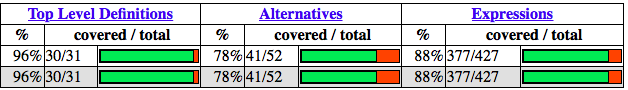
\includegraphics[scale=0.38]{coverage.png}
\caption{Test Coverage Results}
\label{fig:test-coverage}
\end{figure}
While not having 100\% of code coverage, our test suite provides a strong evidence that proposed semantics enjoys
opacity by exercising them on randomly generated programs of increasing size. By analysing test coverage
results, we can observe that code not reached by test cases consists of stuck states on program semantics.

For generating random programs we use basic generators provided by QuickCheck library and build \ensuremath{\TC{Arbitrary}}
instances for \ensuremath{\D{Tran}} and \ensuremath{\D{Proc}} types. Below, we present a snippet of instance for \ensuremath{\D{Proc}}. Code for \ensuremath{\D{Tran}}
follows the same structure.
\begin{hscode}\SaveRestoreHook
\column{B}{@{}>{\hspre}l<{\hspost}@{}}%
\column{3}{@{}>{\hspre}l<{\hspost}@{}}%
\column{4}{@{}>{\hspre}l<{\hspost}@{}}%
\column{5}{@{}>{\hspre}l<{\hspost}@{}}%
\column{6}{@{}>{\hspre}l<{\hspost}@{}}%
\column{8}{@{}>{\hspre}l<{\hspost}@{}}%
\column{12}{@{}>{\hspre}l<{\hspost}@{}}%
\column{14}{@{}>{\hspre}l<{\hspost}@{}}%
\column{E}{@{}>{\hspre}l<{\hspost}@{}}%
\>[B]{}\mathkw{instance}\;\TC{Arbitrary}\;\D{Proc}\;\mathkw{where}{}\<[E]%
\\
\>[B]{}\hsindent{3}{}\<[3]%
\>[3]{}\F{arbitrary}{}\<[E]%
\\
\>[3]{}\hsindent{2}{}\<[5]%
\>[5]{}\mathrel{=}\F{sized}\;\F{genProc}{}\<[E]%
\\[\blanklineskip]%
\>[B]{}\F{genProc}\mathbin{::}\D{Int}\to \D{Gen}\;\D{Proc}{}\<[E]%
\\
\>[B]{}\F{genProc}\;\V{n}{}\<[E]%
\\
\>[B]{}\hsindent{4}{}\<[4]%
\>[4]{}\mid \V{n}\leq \C{0}\mathrel{=}\C{PVal}\F{\,\langle\$\rangle\,}\F{arbitrary}{}\<[E]%
\\
\>[B]{}\hsindent{4}{}\<[4]%
\>[4]{}\mid \F{otherwise}{}\<[E]%
\\
\>[4]{}\hsindent{4}{}\<[8]%
\>[8]{}\mathrel{=}\F{frequency}\;{}\<[E]%
\\
\>[8]{}\hsindent{4}{}\<[12]%
\>[12]{}[\mskip1.5mu {}\<[E]%
\\
\>[12]{}\hsindent{2}{}\<[14]%
\>[14]{}(\V{n}\mathbin{+}\C{1},\C{PVal}\F{\,\langle\$\rangle\,}\F{arbitrary}){}\<[E]%
\\
\>[8]{}\hsindent{4}{}\<[12]%
\>[12]{},(\V{n2},\C{PFork}\F{\,\langle\$\rangle\,}\F{genProc}\;(\V{n}\mathbin{-}\C{1})){}\<[E]%
\\
\>[8]{}\hsindent{4}{}\<[12]%
\>[12]{},(\V{n2},\C{PAt}\;\C{Nothing}\F{\,\langle\$\rangle\,}\F{arbitrary}){}\<[E]%
\\
\>[8]{}\hsindent{4}{}\<[12]%
\>[12]{},(\V{n},(\C{\,\oplus_P\,})\F{\,\langle\$\rangle\,}\F{genProc}\;\V{n2}\F{\,\langle *\rangle\,}\F{genProc}\;\V{n2}){}\<[E]%
\\
\>[8]{}\hsindent{4}{}\<[12]%
\>[12]{}\mskip1.5mu]{}\<[E]%
\\
\>[4]{}\hsindent{2}{}\<[6]%
\>[6]{}\mathkw{where}{}\<[E]%
\\
\>[6]{}\hsindent{2}{}\<[8]%
\>[8]{}\V{n2}\mathrel{=}\F{div}\;\V{n}\;\C{2}{}\<[E]%
\ColumnHook
\end{hscode}\resethooks
The \ensuremath{\F{sized}} function allows for generating values with a size limit and \ensuremath{\F{frequency}} creates a generator
that chooses each alternative with a probability proportional to the accompanying weight.

The TL2-based semantics passed in all tests for safety properties, as expected, since it is well-known
that TL2 provides opacity. But, the semantics based on STM-Haskell does not enjoy such safety properties
since it allows the reading from an inconsistent view of memory. Next example shows how such invalid
memory access can happen.

\begin{Example}
Consider the following program, where \ensuremath{\V{x}} is some variable:
\begin{hscode}\SaveRestoreHook
\column{B}{@{}>{\hspre}l<{\hspost}@{}}%
\column{E}{@{}>{\hspre}l<{\hspost}@{}}%
\>[B]{}\V{t1}\mathbin{::}\D{Tran}{}\<[E]%
\\
\>[B]{}\V{t1}\mathrel{=}\C{TRead}\;\V{x}\C{\,\oplus_T\,}\C{TRead}\;\V{x}\C{\,\oplus_T\,}\C{TRead}\;\V{x}{}\<[E]%
\\[\blanklineskip]%
\>[B]{}\V{t2}\mathbin{::}\D{Tran}{}\<[E]%
\\
\>[B]{}\V{t2}\mathrel{=}\C{TWrite}\;\V{x}\;\V{v}{}\<[E]%
\\[\blanklineskip]%
\>[B]{}\V{p}\mathbin{::}\D{Proc}{}\<[E]%
\\
\>[B]{}\V{p}\mathrel{=}\V{Fork}\;(\C{PAt}\;\C{Nothing}\;\V{t1})\C{\,\oplus_P\,}\V{Fork}\;(\C{PAt}\;\C{Nothing}\;\V{t2}){}\<[E]%
\ColumnHook
\end{hscode}\resethooks
One of the possible executions of \ensuremath{\V{p}} using STM-Haskell semantics would result in the following
history:
\begin{hscode}\SaveRestoreHook
\column{B}{@{}>{\hspre}l<{\hspost}@{}}%
\column{4}{@{}>{\hspre}l<{\hspost}@{}}%
\column{E}{@{}>{\hspre}l<{\hspost}@{}}%
\>[4]{}[\mskip1.5mu \C{IBegin}\;\C{1},\C{IBegin}\;\C{2},\C{IRead}\;\C{1}\;\V{x}\;\C{0}{}\<[E]%
\\
\>[4]{},\C{IWrite}\;\C{2}\;\V{x}\;\C{10},\C{IRead}\;\C{1}\;\V{x}\;\C{0},\C{ICommit}\;\C{2}{}\<[E]%
\\
\>[4]{},\C{IRead}\;\C{1}\;\V{x}\;\C{0},\mathbin{...}\mskip1.5mu]{}\<[E]%
\ColumnHook
\end{hscode}\resethooks
which violates opacity because it does allow transaction \ensuremath{\V{t1}} to read from an inconsistent
memory view. On TL2 semantics safety is preserved because when transaction \ensuremath{\V{t1}} tries to
execute third read it would be aborted.
\end{Example}

\section{Related Work}\label{sec:related}

\paragraph{Semantics for STM:}
Semantics for STM have been received a considerable attention recently~\cite{Harris05,Abadi2011,Moore2008,Liblit06}.
Harris et al.~\cite{Harris05} defines a stop-the-world operational semantics for STM Haskell.
Essentially, Harris uses a multi-step execution model for transaction execution that does not
allows the investigation of safety property neither how interleaving of transactions happens.
Such approach for STM semantics does not allows the investigation of safety properties in terms
of execution histories, since no interleaving between transactions happen.

Abadi et. al.~\cite{Abadi2011} developed the so-called calculus of automatic mutual exclusion (AME) and
shows how to model the behavior of atomic blocks. Using AME they model STM systems that use
in-place update, optimistic concurrency, lazy-conflict detection and roll-back and determine assumptions
that ensure correctness criteria. As~\cite{Abadi2011}, our work defines
different semantics for the same language with the intent to verify STM algorithms, but they use manual proofs
to assert that their semantics enjoy criteria of interest and our work advocates the use of automated testing
tools to early discover semantic design failures before starting proofs.

Moore et. al.~\cite{Moore2008} proposes a series of languages that model several behaviors of STM. Such
models abstract implementation details and provide high-level definitions. Moore uses small-step operational semantics
to explicitly model interleving execution of threads. Manual proofs of isolation properties are described as a
techinical report~\cite{Moore2008a}.

\paragraph{Safety properties for STM:} Safety criteria for STM was another line of research pursued
recently~\cite{LesaniP14,Guerraoui2008}. Opacity was defined by Guerraoui et. al.~\cite{Guerraoui2008}
and it is described as a condition on generated histories by a TM algorithm and provide a graph-based
characterization of opacity. Such graph is built from histories and an algorithm is considered opaque if
the corresponding graph is acyclic for every possible history. Lesani et. al.~\cite{LesaniP14} describes
an equivalent safety property called markability, which decomposes opacity in three invariants and prove
that these invariants are equivalent to opacity. 


\paragraph{Formal verification of STM:} Formal verification of STM algorithms has been an active subject
of recent research~\cite{Lesani2012,CohenPZ08,cohen2007,Guerraoui2008a,Lesani2013}. Lehsani et.al.~\cite{Lesani2012}
describes a PVS~\cite{Owre1992} formalization of a framework for verifying STM algorithms based on I/O automata. The
main idea of Lehsani's framework is to represent both specifications and algorithms as automata and their equivalence is
verified by proving a simulation relation between these automata. The use of model checker to verify TM algorithms was
the subject of~\cite{CohenPZ08,cohen2007}. Both works use the specification languages of model checkers~\cite{Lamport2002}
to describe STM implementations and check them against safety properties. 
We leave using proof assistants for verifying safety properties of our STM semantics for future work.


\paragraph{Testing algorithms for STM:} Automated testing for a compiler of a STM high-level language to
a virtual machine was the subject of~\cite{Hu08}. He uses QuickCheck to generate random high-level STM
programs and check that their virtual machine compiler preserves the semantics of source programs. Unlike our work that
focus on verifying safety of algorithms expressed as small-step operational semantics, Hu et. al. concerns only with
semantic preservation of compilation process and uses multi-steps to evaluate transactions in a stop-the-world semantics for
their high-level language. While such semantics design choices are reasonable for verifying a semantic preservation theorem for a compiler,
they do allow for checking safety properties. Harmanci et. al.~\cite{Harmanci2009} describes a tool for testing
TM algorithms, called TM-unit. Using TM-unit domain specific language, users can specify TM workloads for both
safety and performance testing of TM algorithms. Authors argue that their domain specific language is simple and
expressive but no formal semantics of this language is provided. We believe that the use of domain specific languages
is invaluable to provide concise and formal specifications of STM algorithm and we leave this line of research for
further work.

\section{Conclusion}\label{sec:conclusion}

In this work we presented safe semantics for a simplied high-level language with STM support and use
property based testing to verify it. The lightweight approach provided by QuickCheck allow us to experiment
with different semantic designs and implementations, and to quickly check any changes. During the development of this work,
we have changed our basic definitions many times, both as a result of correcting errors, and streamlining the presentation.
Ensuring that our changes were consistent was simply a matter of re-running test suite. Encoding safety properties as
Haskell functions over STM histories provides a clean and concise implementation that helps not only to fix semantics
but also to improve our understanding of STM algorithms.

As future work we intend to use Agda~\cite{Norell2009} to provide formally certified proofs that the presented semantics does
enjoy safety properties and also investigate the usage of domain specific languages to ease the task of specifying algorithms
as small-step operational semantics of a simple transactional language.


\bibliographystyle{ACM-Reference-Format}
\bibliography{references} 

\end{document}
